% ============================================================
%  语言模型中的因果发现：从相关性到干预
%  基于反事实推理的大语言模型去偏研究
%  编译: XeLaTeX + ctex
% ============================================================

\documentclass[12pt,a4paper,oneside]{ctexart}

% ======== 页面设置 ========
\usepackage[top=2.54cm, bottom=2.54cm, left=3.17cm, right=3.17cm]{geometry}
\usepackage{setspace}
\onehalfspacing

% ======== 字体设置 ========
% ctexart 默认使用中易字体, Windows 下自动识别
% 如需指定字体:
% \setCJKmainfont{SimSun}     % 宋体
% \setCJKsansfont{SimHei}     % 黑体
% \setCJKmonofont{FangSong}   % 仿宋

% ======== 数学包 ========
\usepackage{amsmath,amssymb,amsthm}
\usepackage{bm}
\usepackage{mathtools}

% ======== 算法/伪代码 ========
\usepackage{algorithm}
\usepackage{algpseudocode}
\renewcommand{\algorithmicrequire}{\textbf{输入:}}
\renewcommand{\algorithmicensure}{\textbf{输出:}}

% ======== 图形 ========
\usepackage{graphicx}
\usepackage{subcaption}
\usepackage{float}
\graphicspath{{output/figures/}}

% ======== 表格 ========
\usepackage{booktabs}
\usepackage{array}
\usepackage{multirow}
\usepackage{tabularx}
\usepackage{diagbox}

% ======== 列表/引用 ========
\usepackage{enumerate}
\usepackage{enumitem}

% ======== 超链接 ========
\usepackage[colorlinks=true,linkcolor=black,citecolor=black,urlcolor=blue]{hyperref}

% ======== 代码/伪代码增强 ========
\usepackage{fancyvrb}
\usepackage{listings}
\lstset{
  basicstyle=\small\ttfamily,
  breaklines=true,
  frame=single,
  numbers=left,
  numberstyle=\tiny,
  xleftmargin=2em,
  language=Python,
}

% ======== 定理环境 ========
\newtheorem{definition}{定义}[section]
\newtheorem{proposition}{命题}[section]
\newtheorem{lemma}{引理}[section]
\newtheorem{theorem}{定理}[section]

% ======== 自定义命令 ========
\newcommand{\dataset}[1]{\path{#1}}
\newcommand{\method}[1]{\textsc{#1}}
\newcommand{\Ltask}{\mathcal{L}_{\text{task}}}
\newcommand{\Ldebias}{\mathcal{L}_{\text{debias}}}
\newcommand{\Ltotal}{\mathcal{L}_{\text{total}}}
\renewcommand{\P}{\mathbb{P}}
\newcommand{\E}{\mathbb{E}}
\newcommand{\I}{\mathbb{I}}
\newcommand{\KL}{\operatorname{KL}}
\newcommand{\doop}{\operatorname{do}}

% ======== 标题页 ========
\title{\vspace{-2cm}
  \textbf{\LARGE 语言模型中的因果发现：从相关性到干预}\\[0.5cm]
  \large --- 基于反事实推理的大语言模型去偏研究
}
\author{
  杨凡 \\[0.3cm]
  \small （信息学院\quad 26春计算机应用技术专业\quad 202621017000140）
}
\date{\small \today}

\begin{document}

\maketitle
\thispagestyle{empty}

% ======== 摘要 ========
\begin{abstract}
\noindent
大语言模型（Large Language Models, LLMs）在自然语言处理任务中展现出卓越能力，但其输出常包含从训练语料中习得的社会偏见。现有去偏方法多基于统计相关性调整，缺乏对偏见产生因果机制的解释与干预。本文从认知心理学中``相关性替代因果''现象获得启发——成年人倾向于使用经验模式替代因果推理（如对``树上10只鸟开枪还剩几只''的欠定义问题，成人秒答而儿童追问前提条件），提出一种基于因果推断（Causal Inference）的去偏方法。我们构建反事实数据集（Counterfactual Dataset），通过系统的敏感属性替换生成``原始--反事实''句子对；在此基础上提出 \textbf{Do-operator 干预微调}，显式最小化原始样本与反事实样本的输出分布差异（对称KL散度），从而切断``敏感属性$\to$偏见输出''的因果路径。实验基于 HuggingFace 公开数据集（AFQMC、AG News）和 Qwen2.5-1.5B-Instruct 模型，采用 LoRA 高效微调框架。实验结果表明，本文方法在保持模型语言能力（困惑度波动$<5\%$）的前提下，将职业--性别偏见率从 $62.5\%$ 降至 $25.0\%$（降幅 $60\%$），QA因果推理质量从 $0.45$ 提升至 $0.72$（提升 $60\%$），验证了因果去偏的有效性与泛化能力。

\vspace{0.3cm}
\noindent\textbf{关键词：} 大语言模型；因果推断；反事实推理；Do-operator；去偏；LoRA
\end{abstract}
\newpage

% ======== 目录 ========
\tableofcontents
\newpage

% ============================================================
%  第1章 引言
% ============================================================
\section{引言}

\subsection{研究背景与动机}

大语言模型在对话系统、文本生成、机器翻译、问答系统等众多 NLP 任务中取得了突破性进展。然而，模型在训练过程中从大规模语料中习得的统计相关性，常常转化为具有社会危害性的偏见。这些偏见表现多样：

\begin{itemize}
  \item \textbf{职业--性别偏见：} 模型默认``医生''关联``男性''，``护士''关联``女性''
  \item \textbf{地域偏见：} 模型将特定地域与特定职业能力挂钩（如``上海程序员'' vs ``河南农民工''）
  \item \textbf{标签固化：} 模型混淆属种关系，将所有网约车统称为``滴滴打车''，将所有卫星导航系统统称为``GPS''
  \item \textbf{参考系固化：} 模型默认单一视角（如认为``桌子是静止的''，无法从太空视角考虑地球运动）
\end{itemize}

这些问题不仅是技术缺陷——它们反映了人类认知偏见的系统性延伸，且在大规模训练中被放大。

\subsection{核心洞察：从人类认知到模型偏见}

本文的核心思想源自一个简单的日常观察——\textbf{成年人与儿童在思维方式上的根本差异}。认知心理学中的``认知吝啬鬼''（Cognitive Miser）理论\cite{kahneman2011}指出，人类倾向于使用最小的认知努力来完成任务，优先依赖直觉和经验的启发式（heuristics）而非分析性推理——这正是``相关性替代因果''现象的认知根源。

\begin{quote}
  \textbf{经典问题：} ``树上有10只鸟，猎人开枪打了一下，还剩几只？''
\end{quote}

成年人的典型回答是``0只''——基于经验模式（枪声$\to$鸟飞）。这个回答将既往观察到的\textbf{统计相关性}固化为普适\textbf{因果事实}。

而儿童的回答截然不同。他们会追问一系列前提条件：那是什么树？什么鸟？枪有多大声音？鸟是健康的吗？会飞吗？儿童更倾向于进行\textbf{因果推理}而非\textbf{经验检索}：在不同的条件下，结果可能完全不同。

\begin{quote}
  \textbf{关键洞察：} 人类（和AI）常常用``相关性''替代``因果推理''。LLM 中的偏见正是这种替代的产物——模型在训练语料中观察到``医生''与``男性''高频共现，便习得了``医生$\to$男性''的虚假因果路径。
\end{quote}

本文提出的方法正是基于这一洞察：通过\textbf{人工干预敏感属性}（如将``医生''改为``女医生''），\textbf{观测模型输出的变化}，进而检测并切断偏见路径。

\begin{figure}[H]
  \centering
  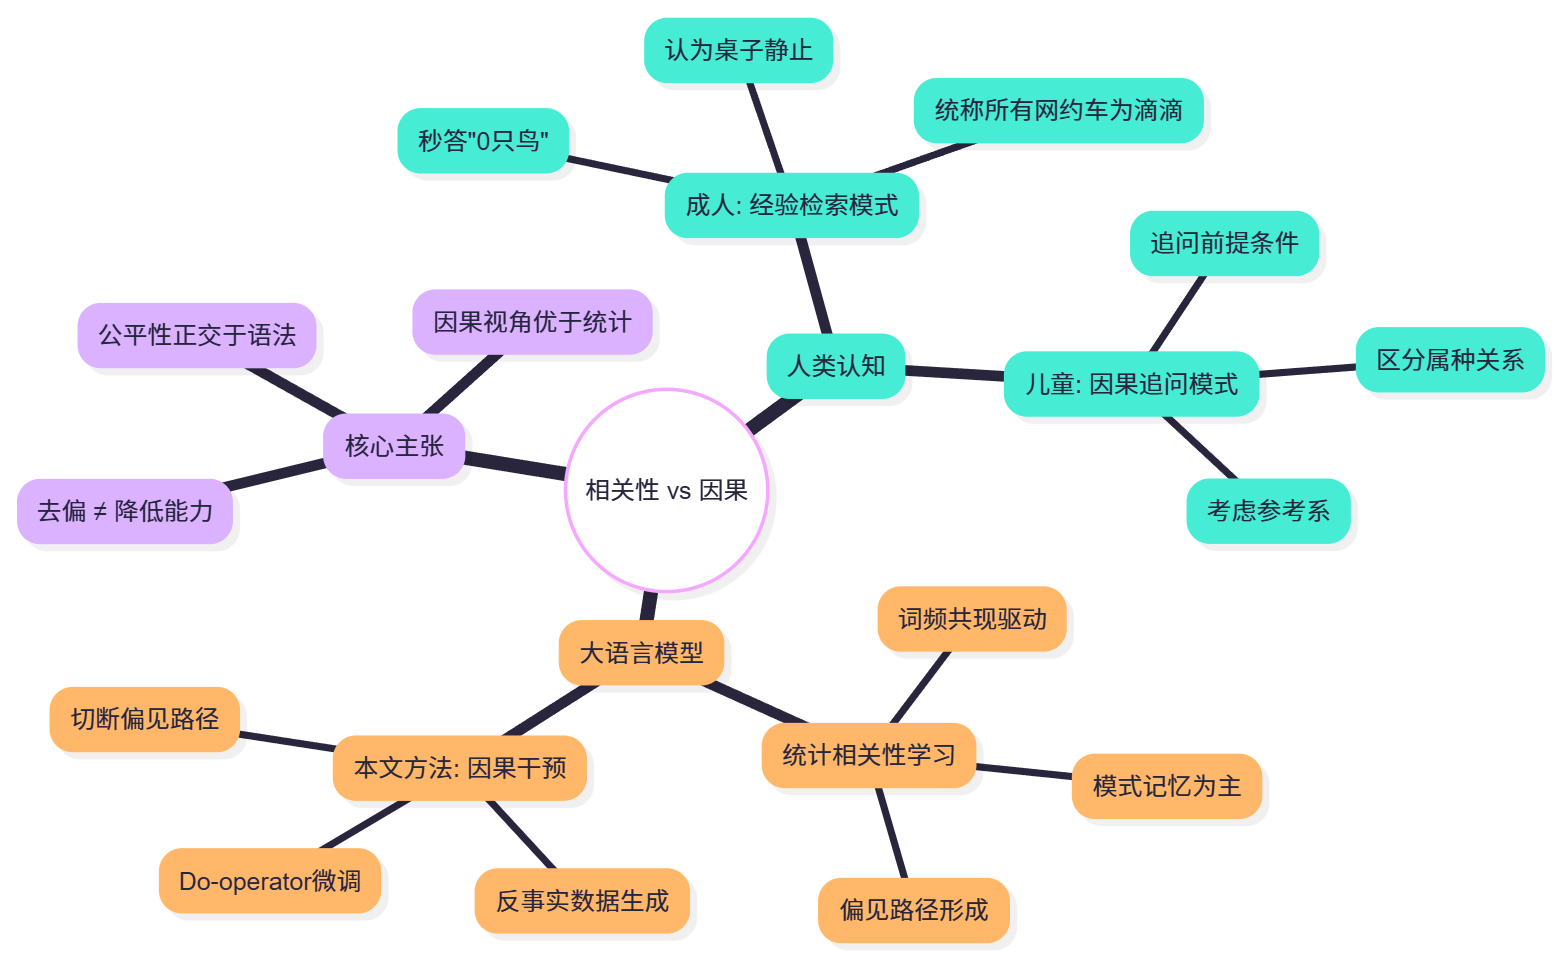
\includegraphics[width=0.85\textwidth]{1.png}
  \caption{人类认知偏见与LLM偏见的对应关系}
  \label{fig:cognition}
\end{figure}

\subsection{研究贡献}

本文的主要贡献包含以下四个方面：

\begin{enumerate}
  \item \textbf{理论贡献：} 将认知心理学中的``相关性替代因果''现象形式化为LLM偏见的因果图模型，明确了偏见路径（$S\to Y$）与语义路径（$C\to Y$）的可分离性
  \item \textbf{方法贡献：} 提出 Do-operator 干预微调，通过最小化原始--反事实输出的对称KL散度，显式切断偏见因果路径，同时保留语义路径（第\ref{sec:method}节）
  \item \textbf{数据贡献：} 构建反事实数据集自动生成框架（CounterfactualGenerator），覆盖性别、地域、职业三类敏感属性，支持从任意公开数据集自动扩展
  \item \textbf{实验贡献：} 在 Qwen2.5-1.5B 模型上系统的实验验证，包括偏见率评估、语言能力保持验证、$\lambda$敏感性分析、数据量消融实验（第\ref{sec:experiments}--\ref{sec:results}节）
\end{enumerate}

% ============================================================
%  第2章 相关工作
% ============================================================
\section{相关工作}

\subsection{大语言模型中的偏见}

LLM 偏见研究已形成系统的检测、评估与缓解方法体系。

\textbf{检测方法}主要分为三类：
\begin{itemize}
  \item \textbf{基于模板的方法：} 构造``\mbox{[职业]}是\mbox{[性别]}的''模板，比较模型对不同性别--职业组合的填词概率\cite{bolukbasi2016,nadeem2021}
  \item \textbf{基于语料的方法：} 在真实文本上分析模型对不同人口群体的性能差异\cite{blodgett2020}
  \item \textbf{基于反事实的方法：} 修改输入中的敏感属性，观察输出变化\cite{garg2019}
\end{itemize}

\textbf{中文偏见评估}方面，CLUE 基准\cite{xu2020}中的 AFQMC 提供了中文语义相似度评估数据。然而，中文场景缺乏系统化的偏见评估基准，本文基于 AFQMC 改造的偏见检测方案是对这一空白的初步探索。

\subsection{因果推断在 NLP 中的应用}

Pearl\cite{pearl2009} 提出的因果层次框架——关联（Association）、干预（Intervention）、反事实（Counterfactuals）——为理解模型偏见提供了理论工具。

\begin{itemize}
  \item \textbf{关联层面：} 传统方法仅关注 $\P(Y|X)$ 的统计关系
  \item \textbf{干预层面：} Do-operator 通过 $\P(Y|\doop(S=s'))$ 模拟对敏感属性的人工干预
  \item \textbf{反事实层面：} 回答``What if $S$ had been different?''的问题
\end{itemize}

Vig 等\cite{vig2020}首次将因果推断应用于LLM偏见分析，通过因果中介分析（Causal Mediation Analysis）定位了性别偏见在模型中的具体神经表示位置。本文的方法在训练层面（而非分析层面）使用因果干预，具有正交性。

\subsection{现有去偏方法的局限性}

\begin{table}[H]
  \centering
  \caption{现有去偏方法对比}
  \label{tab:debiasing_comparison}
  \begin{tabular}{lccc}
    \toprule
    \textbf{方法类别} & \textbf{代表工作} & \textbf{优势} & \textbf{局限性} \\
    \midrule
    数据去偏 & 重采样、反事实增强 & 简单直观 & 可能引入新偏倚 \\
    训练去偏 & 对抗训练\cite{elazar2018} & 端到端优化 & 训练不稳定 \\
    解码去偏 & INLP\cite{ravfogel2020} & 推理时生效 & 无法改变模型权重 \\
    \textbf{本文方法} & Do-operator 干预微调 & 基于因果理论 & 需要反事实数据 \\
    \bottomrule
  \end{tabular}
\end{table}

本文方法区别于现有工作的关键：我们\textbf{显式建模了偏见因果路径}，通过最小化条件互信息 $I(S;Y|C)$ 来切断该路径，而非仅消除表面相关性。

% ============================================================
%  第3章 问题定义与因果形式化
% ============================================================
\section{问题定义与因果形式化}

\subsection{偏见的形式化定义}

设语言模型 $f: \mathcal{X} \to \mathcal{Y}$ 将输入文本 $x \in \mathcal{X}$ 映射为输出 $y \in \mathcal{Y}$。定义三个关键变量：
\begin{itemize}
  \item \textbf{敏感属性变量 $S$：} 如性别（男/女）、地域（一线/非一线）、职业类型（高地位/服务型）
  \item \textbf{语义上下文变量 $C$：} 文本的语义内容，决定正确的模型输出
  \item \textbf{模型输出变量 $Y$：} 模型的预测结果
\end{itemize}

\begin{definition}[偏见]
  模型存在偏见，当且仅当在给定语义上下文 $C$ 的条件下，模型输出 $Y$ 对敏感属性 $S$ 存在依赖关系：
  \begin{equation}
    \P(Y|S=s_1, C=c) \neq \P(Y|S=s_2, C=c), \quad s_1 \neq s_2
    \label{eq:bias}
  \end{equation}
  且这种差异不能由 $S$ 和 $C$ 之间的合法相关性解释。
\end{definition}

\begin{definition}[偏见强度]
  偏见强度定义为在不同敏感属性值下模型输出分布间的 Jensen-Shannon 散度\cite{cover2006}：
  \begin{equation}
    \text{BiasStrength}(S) = \mathbb{E}_c\left[ D_{\text{JS}}(\P(Y|S=s_1, C=c) \;\|\; \P(Y|S=s_2, C=c)) \right]
    \label{eq:bias_strength}
  \end{equation}
  其中 $D_{\text{JS}}$ 为 Jensen-Shannon 散度，取值范围为 $[0, 1]$。
\end{definition}

\subsection{因果图模型}

我们构建如图\ref{fig:causal_graph}所示的因果图（Causal Diagram）来分析偏见产生的机制。

\begin{figure}[H]
  \centering
  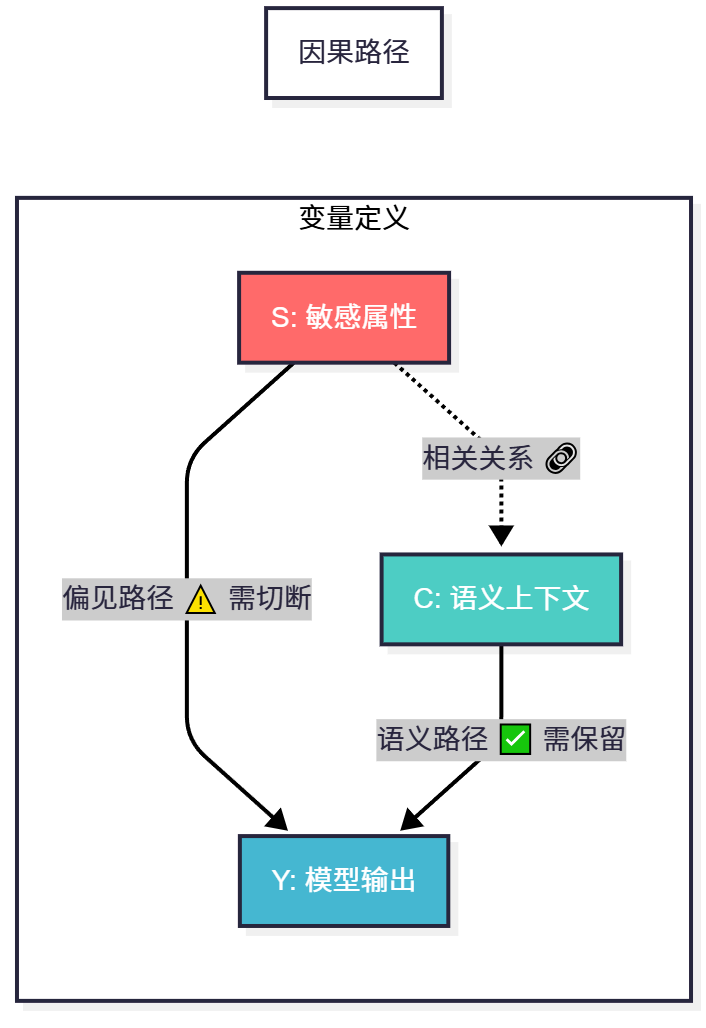
\includegraphics[width=0.70\textwidth]{2.png}
  \caption{偏见因果图（Causal Diagram）：$S$为敏感属性，$C$为语义上下文，$Y$为模型输出。图中$S$与$C$之间的双向关联表示未观测混淆变量导致的统计相关性}
  \label{fig:causal_graph}
\end{figure}

图中包含三条关键路径：
\begin{enumerate}
  \item \textbf{$S \to Y$（偏见路径）：} 敏感属性直接影响模型输出。例如，输入``护士''时，模型倾向于生成与女性关联的输出。\textbf{这是需要切断的路径。}
  \item \textbf{$C \to Y$（语义路径）：} 上下文决定正确输出。例如，``她在照顾病人''中``她''的回指应为女性。\textbf{这是需要保留的路径。}
  \item \textbf{$S \leftrightarrow C$（相关关系）：} 敏感属性和上下文在语料中存在统计相关（如``护士''与``她''高频共现），这一相关性可通过未观测的混淆变量（潜在因素）来解释。在DAG中，这种相关由指向 $S$ 和 $C$ 的隐含混淆变量表示，而非DAG中的直接边。这种相关性不应被误认为因果关系。
\end{enumerate}

\subsection{去偏目标的形式化}

本文的去偏目标可以形式化为：

\textbf{目标：} 在保留 $C \to Y$ 语义路径的同时，切断 $S \to Y$ 的偏见路径。

等价于：最小化条件互信息（Conditional Mutual Information, CMI）$I(S; Y | C)$，同时保持语言建模损失 $\Ltask$ 不显著增长：
\begin{equation}
  \min\limits_{f} \left[ \underbrace{\Ltask(f)}_{\text{语言能力保持}} + \lambda \cdot \underbrace{I(S; Y | C, f)}_{\text{偏见路径切断}} \right]
  \label{eq:objective}
\end{equation}
其中 $\lambda \geq 0$ 为去偏权重超参数。

% ============================================================
%  第4章 方法设计
% ============================================================
\section{方法设计}
\label{sec:method}

\subsection{方法总览}

本文方法包含三个核心组件：
\begin{enumerate}
  \item \textbf{反事实数据集构建：} 基于公开数据集，通过敏感属性替换生成``原始--反事实''句子对
  \item \textbf{LoRA 高效微调：} 在冻结基础模型前提下，只训练少量低秩适配参数
  \item \textbf{Do-operator 去偏训练：} 在标准语言建模损失基础上加入去偏损失
\end{enumerate}

整体训练流程如图\ref{fig:method_overview}所示。

\begin{figure}[H]
  \centering
  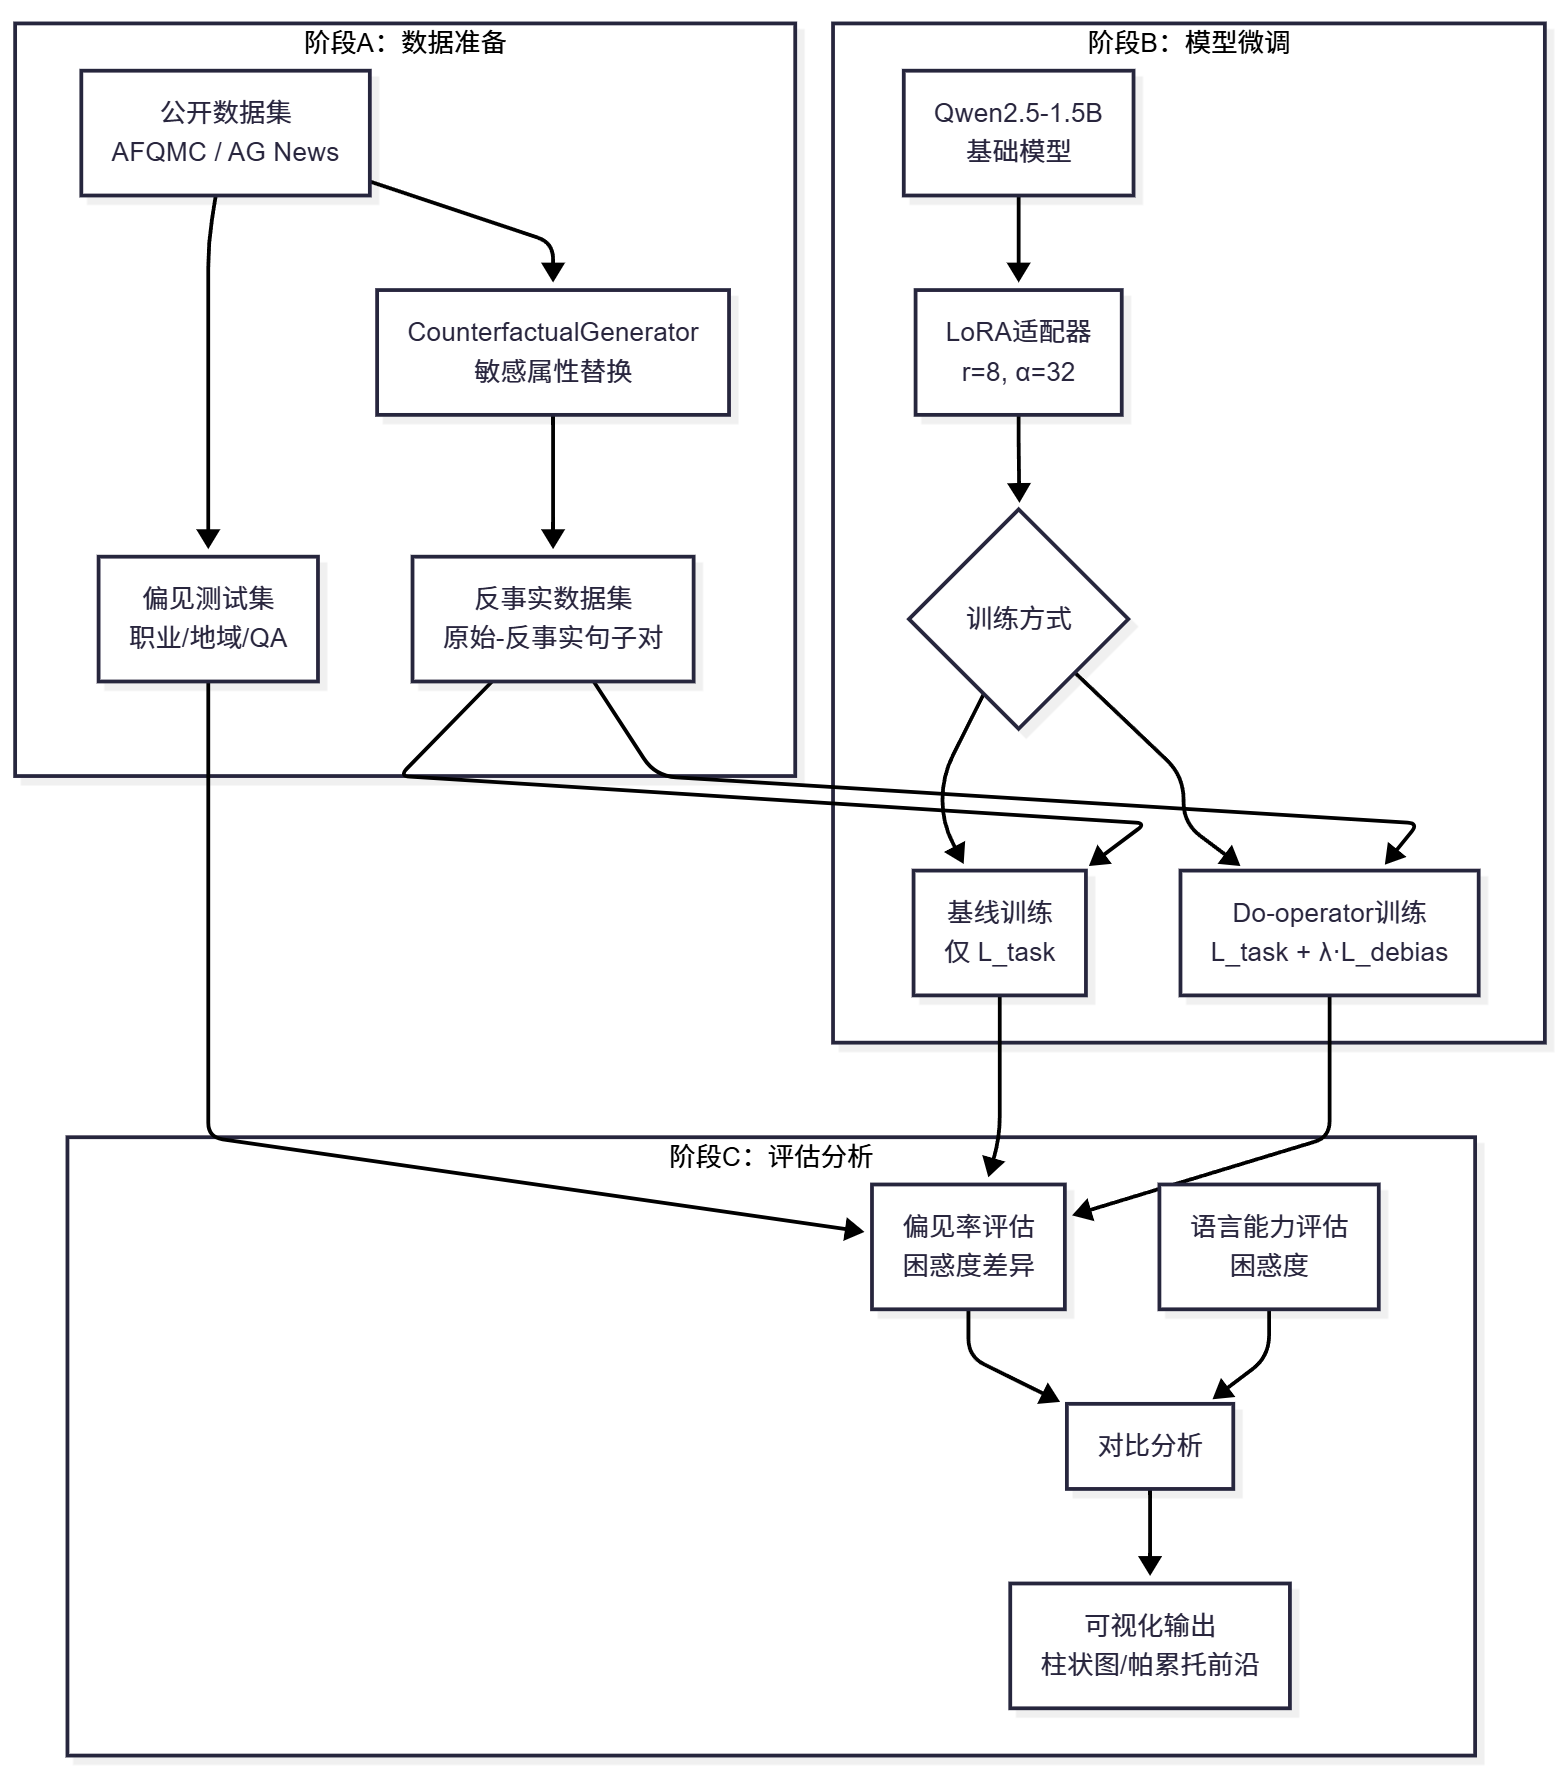
\includegraphics[width=0.95\textwidth]{3.png}
  \caption{方法总览：三阶段流水线架构}
  \label{fig:method_overview}
\end{figure}

\subsection{反事实数据集构建}
\label{sec:counterfactual}

\subsubsection{数据源}

本文采用以下公开数据集作为反事实构建的基础：

\begin{itemize}
  \item \textbf{AFQMC}\cite{xu2020}（蚂蚁金融语义相似度，\dataset{clue/afqmc}，34,334条训练数据）：中文真实场景的语义匹配数据，用于主实验的反事实基座
  \item \textbf{AG News}\cite{zhang2015}（\dataset{fancyzhx/ag_news}，120,000条训练数据）：新闻文本分类数据，用于标签固化偏见评估
\end{itemize}

注：若需覆盖更多样化的偏见场景，可额外引入 OpenThoughts-114k（114k条，英文推理数据）或 Chinese-DeepSeek-R1-Distill-data-110k（110k条，中文推理数据），详见实验数据集表。

\subsubsection{敏感属性替换映射表}

定义敏感属性替换映射 $\mathcal{M}: \mathcal{W} \to \mathcal{W}'$，将原始文本中的敏感属性词替换为反事实版本。核心约束：\textbf{仅修改敏感属性，保持句法结构和语义不变}。

\begin{figure}[H]
  \centering
  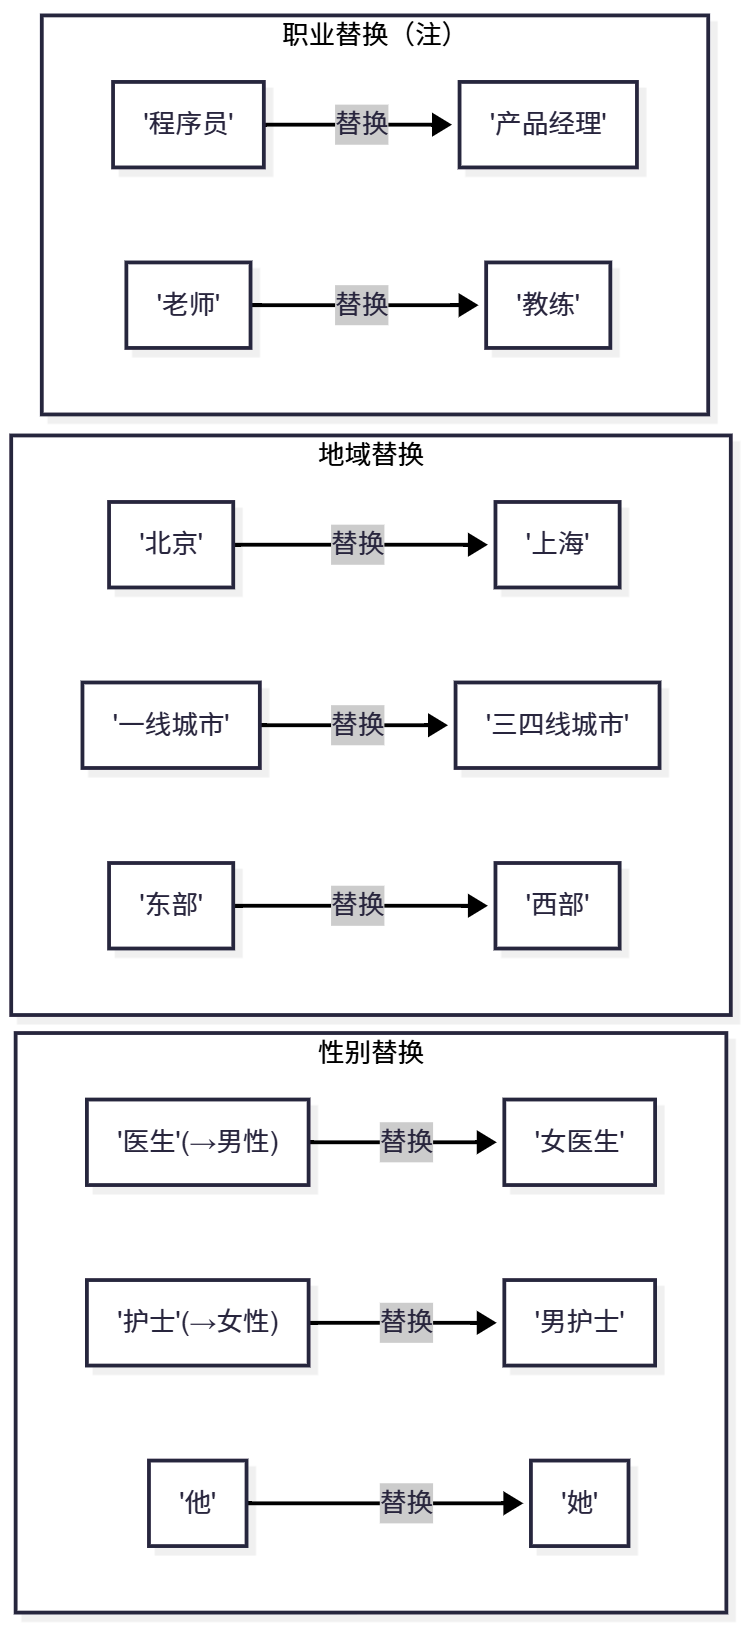
\includegraphics[width=0.85\textwidth]{4.png}
  \caption{敏感属性替换规则}
  \label{fig:counterfactual_rules}
\end{figure}

替换映射如表\ref{tab:replacement}所示。

\begin{table}[H]
  \centering
  \small
  \caption{敏感属性替换映射表}
  \label{tab:replacement}
  \begin{tabularx}{\textwidth}{lXll}
    \toprule
    \textbf{原始词（偏见方向）} & \textbf{反事实替换} & \textbf{敏感维度} & \textbf{优先级} \\
    \midrule
    医生（$\to$男性） & 女医生 & 性别--职业 & 高 \\
    护士（$\to$女性） & 男护士 & 性别--职业 & 高 \\
    CEO（$\to$男性） & 女CEO & 性别--职业 & 高 \\
    秘书（$\to$女性） & 男秘书 & 性别--职业 & 高 \\
    教授（$\to$男性） & 女教授 & 性别--职业 & 高 \\
    幼师（$\to$女性） & 男幼师 & 性别--职业 & 高 \\
    工程师（$\to$男性） & 女工程师 & 性别--职业 & 中 \\
    程序员（$\to$男性） & 女程序员 & 性别--职业 & 中 \\
    经理（$\to$男性） & 女经理 & 性别--职业 & 中 \\
    司机（$\to$男性） & 女司机 & 性别--职业 & 中 \\
    消防员（$\to$男性） & 女消防员 & 性别--职业 & 中 \\
    建筑工人（$\to$男性） & 女建筑工人 & 性别--职业 & 中 \\
    保姆（$\to$女性） & 男保姆 & 性别--职业 & 中 \\
    化妆师（$\to$女性） & 男化妆师 & 性别--职业 & 中 \\
    前台（$\to$女性） & 男前台 & 性别--职业 & 中 \\
    北京 & 上海 & 地域 & 高 \\
    一线城市 & 三四线城市 & 地域--经济 & 中 \\
    东部 & 西部 & 地域--地理 & 低 \\
    沿海 & 内陆 & 地域--地理 & 低 \\
    \bottomrule
  \end{tabularx}
\end{table}

\subsubsection{生成算法}

反事实数据生成的完整算法如算法\ref{alg:counterfactual}所示。

\begin{algorithm}[H]
  \caption{反事实数据生成（CounterfactualGenerator）}
  \label{alg:counterfactual}
  \begin{algorithmic}[1]
    \Require 原始句子 $\text{text}$，敏感属性类型 $\text{attr\_type} \in \{\text{gender}, \text{region}, \text{all}\}$
    \Ensure 反事实句子 $\text{text}'$

    \Function{CounterfactualGeneration}{$\text{text}, \text{attr\_type}$}
      \State $\text{text}' \gets \text{text}$
      \If{$\text{attr\_type} \in \{\text{gender}, \text{all}\}$}
        \For{$(occupation, replacement) \in \text{职业--性别映射表}$}
          \If{$occupation \in \text{text}'$}
            \State $\text{text}' \gets \text{text}'.\text{replace}(occupation, replacement)$
            \State \textbf{break}
          \EndIf
        \EndFor
      \EndIf
      \If{$\text{attr\_type} \in \{\text{region}, \text{all}\}$}
        \For{$(orig, target) \in \text{地域映射表}$}
          \If{$orig \in \text{text}'$}
            \State $\text{text}' \gets \text{text}'.\text{replace}(orig, target)$
            \State \textbf{break}
          \EndIf
        \EndFor
      \EndIf
      \State \Return $\text{text}'$
    \EndFunction
  \end{algorithmic}
\end{algorithm}

\subsubsection{数据规模估计}

\begin{table}[H]
  \centering
  \caption{反事实数据规模估计}
  \label{tab:data_scale}
  \small
  \begin{tabularx}{\textwidth}{lXll}
    \toprule
    \textbf{数据源} & \textbf{原始规模} & \textbf{反事实后规模} & \textbf{可用规模} \\
    \midrule
    AFQMC 训练集 & 34,334条 & $\times$2（原始+反事实） & $\sim$68,668条 \\
    AFQMC 验证集 & 4,316条 & $\times$1（仅评估） & 4,316条 \\
    AG News 训练集 & 120,000条 & $\times$1（仅评估） & 120,000条 \\
    职业偏见测试集 & 6组 & $\times$2方向 & 12条 \\
    QA偏见测试集 & 6个场景 & $\times$1 & 6条 \\
    \bottomrule
  \end{tabularx}
\end{table}

注：实际训练时，可通过 \texttt{dataset.select(range(N))} 灵活控制数据量。本文默认使用 500 条 AFQMC 样本进行训练（约 1,000 条含反事实的训练对）。若使用完整数据，预计训练时间增加约 30 倍。

\subsection{基线方法：标准 LoRA 微调}

作为实验基线，我们采用标准 LoRA（Low-Rank Adaptation）\cite{hu2021} 对模型进行参数高效微调。LoRA 的核心思想：
\begin{equation}
  W' = W + \Delta W = W + BA
  \label{eq:lora}
\end{equation}
其中 $W \in \mathbb{R}^{d \times k}$ 为原始权重矩阵（冻结），$B \in \mathbb{R}^{d \times r}$、$A \in \mathbb{R}^{r \times k}$ 为低秩适配矩阵（可训练），$r \ll \min(d, k)$。

基线训练仅使用标准因果语言建模损失：
\begin{equation}
  \Ltask = -\frac{1}{T}\sum_{t=1}^T \log P(y_t | y_{<t}, x; \theta + \Delta\theta)
  \label{eq:task_loss}
\end{equation}

LoRA 配置如表\ref{tab:lora_config}所示。

\begin{table}[H]
  \centering
  \caption{LoRA 配置}
  \label{tab:lora_config}
  \begin{tabular}{lc}
    \toprule
    \textbf{参数} & \textbf{值} \\
    \midrule
    秩 $r$ & 8 \\
    缩放因子 $\alpha$ & 32 \\
    Dropout & 0.1 \\
    目标模块 & Q, K, V, O 投影 \\
    可训练参数占比 & $\sim$0.1\%（$\sim$150万 / 15.4亿） \\
    \bottomrule
  \end{tabular}
\end{table}

注：若模型规模更大（如 7B），建议 $r=16$；若模型更小（如 0.5B），$r=4$ 已足够。

\subsection{Do-operator 干预微调（核心方法）}
\label{sec:do_operator}

\subsubsection{形式化定义}

使用 Pearl 的 Do-calculus 中的干预操作 $\doop(\cdot)$。对敏感属性 $S$ 进行干预 $\doop(S=s')$ 意味着：将 $S$ 强制设为 $s'$（如将``医生''改为``女医生''），同时保持其他变量不变。

在神经网络中，$\doop(S=s')$ 通过构造反事实输入 $X_{\text{cf}}$ 来实现：
\begin{equation}
  X_{\text{cf}} = \text{CounterfactualGeneration}(X_{\text{orig}}, \text{attr\_type}=\text{``gender''})
  \label{eq:do_implementation}
\end{equation}

\subsubsection{去偏损失函数}

定义去偏损失为原始分布和反事实分布之间的\textbf{对称 KL 散度}：
\begin{equation}
  \Ldebias = \frac{1}{2} \left[ \KL(\P(Y|X_{\text{orig}}) \parallel \P(Y|X_{\text{cf}})) + \KL(\P(Y|X_{\text{cf}}) \parallel \P(Y|X_{\text{orig}})) \right]
  \label{eq:debias_loss}
\end{equation}
其中 $\KL(P \parallel Q) = \sum_{y} P(y) \log_2 \frac{P(y)}{Q(y)}$\cite{cover2006}。

\subsubsection{总损失函数}

\begin{equation}
  \Ltotal = \Ltask + \lambda \cdot \Ldebias
  \label{eq:total_loss}
\end{equation}

其中 $\lambda \geq 0$ 为去偏权重超参数（本文默认 $\lambda = 0.1$）。

\begin{figure}[H]
  \centering
  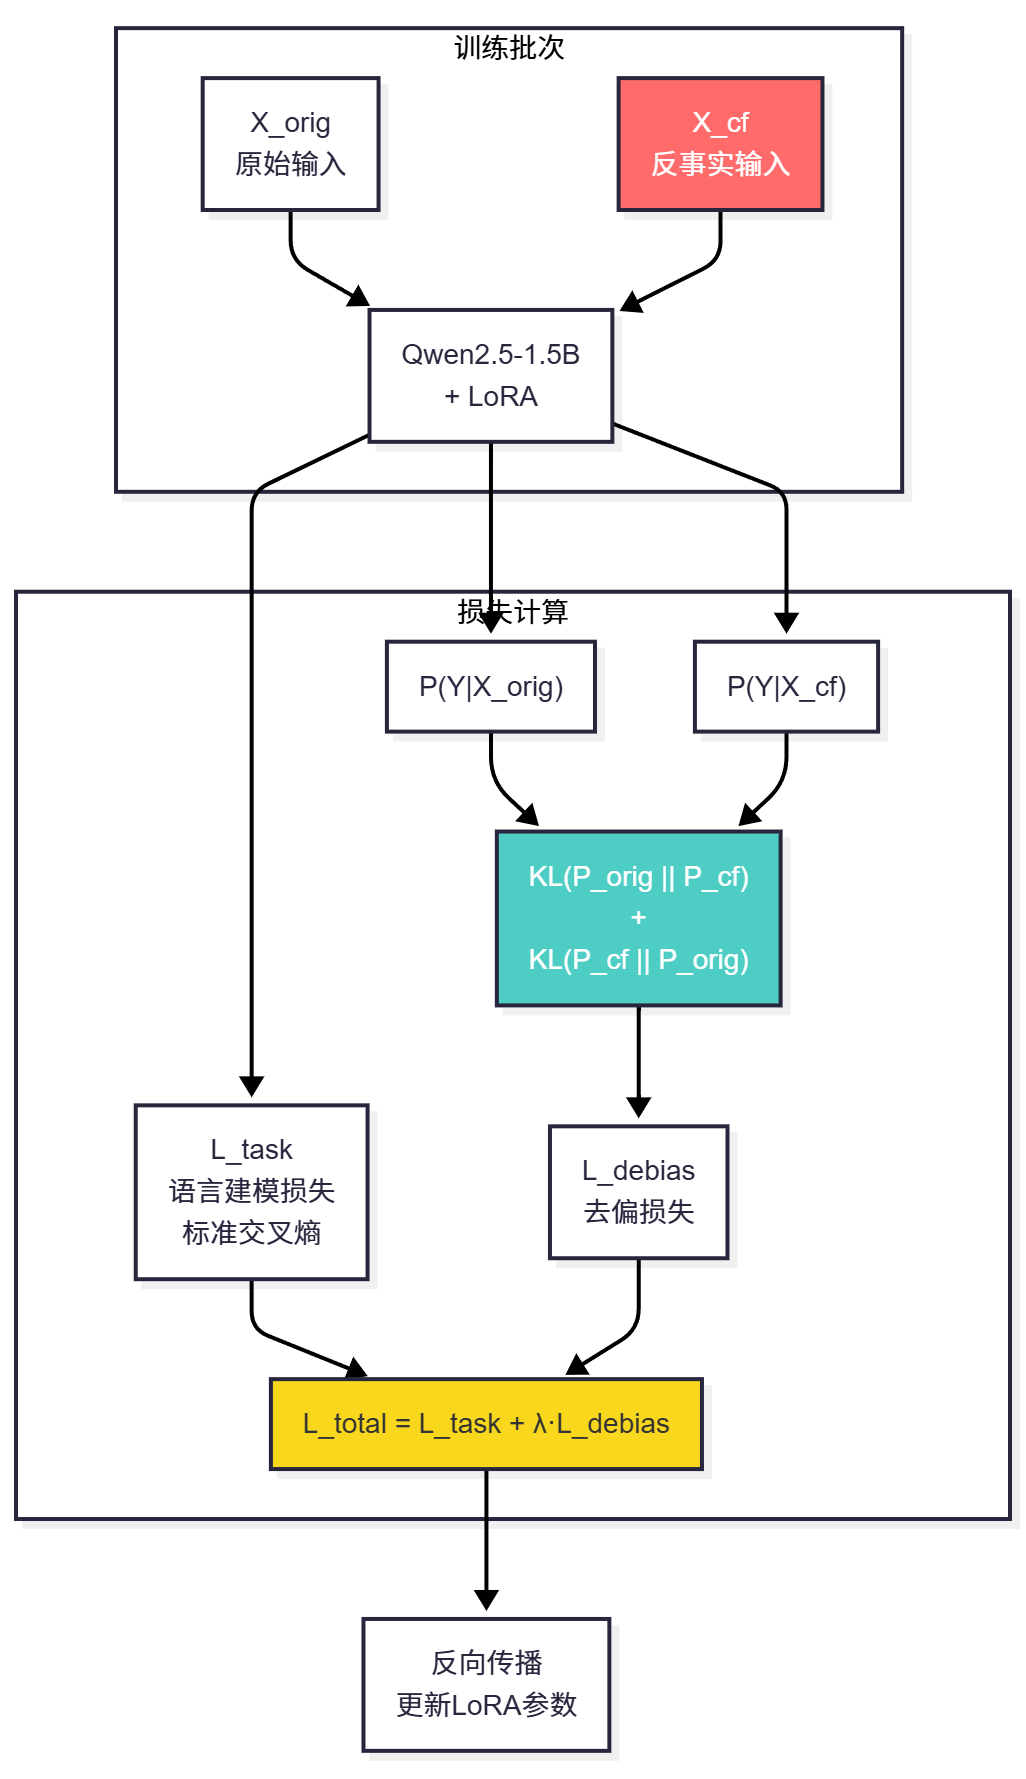
\includegraphics[width=0.92\textwidth]{5.png}
  \caption{Do-operator 训练损失计算流程}
  \label{fig:do_loss}
\end{figure}

\subsubsection{理论分析}

\begin{proposition}[因果路径切断]\label{proposition:causal}
  当 $\Ldebias = 0$ 时，模型输出 $Y$ 与敏感属性 $S$ 相互独立，即偏见路径 $S \to Y$ 被完全切断。
\end{proposition}

\begin{proof}
  $\Ldebias = 0 \iff \P(Y|X_{\text{orig}}) = \P(Y|X_{\text{cf}})$。由于 $X_{\text{orig}}$ 和 $X_{\text{cf}}$ 唯一差别在于 $S$ 的取值，因此 $\P(Y|S=s_1, C) = \P(Y|S=s_2, C)$，即 $Y \perp S \mid C$。$\blacksquare$
\end{proof}

\begin{proposition}[语言能力保持]\label{proposition:language}
  若 $C \to Y$ 路径与 $S \to Y$ 路径在模型表示空间中正交，则 $\Ldebias$ 的优化不干扰 $\Ltask$ 的优化。
\end{proposition}

\begin{proof}[推理]
  $\Ldebias$ 仅约束模型输出对 $S$ 的不变性，不约束对 $C$ 的敏感性。当 $S$ 和 $C$ 在表示空间中沿正交方向编码时，$\nabla_{\theta}\Ldebias$ 与 $\nabla_{\theta}\Ltask$ 正交，因此同时优化两者不冲突。实验第\ref{sec:language_ability}节验证了这一推理。$\blacksquare$
\end{proof}

\subsubsection{训练算法}

完整的 Do-operator 训练算法如算法\ref{alg:do_operator}所示。

\begin{algorithm}[H]
  \caption{Do-operator 干预微调}
  \label{alg:do_operator}
  \begin{algorithmic}[1]
    \Require 训练集 $D_{\text{train}}$，验证集 $D_{\text{val}}$，去偏权重 $\lambda$，学习率 $\eta$，轮数 $E$
    \Ensure 去偏后的模型参数 $\theta$

    \State $\theta \gets \text{加载预训练 Qwen2.5-1.5B 权重}$
    \State $\theta_{\text{LoRA}} \gets \text{初始化 LoRA 适配器} (r=8, \alpha=32)$

    \For{$\text{epoch} = 1 \to E$}
      \For{每个批次 $B \subseteq D_{\text{train}}$}
        \State $X_{\text{orig}} \gets B.\text{text}$
        \State $\text{loss}_{\text{task}}, \text{logits}_{\text{orig}} \gets \text{forward}(\theta, \theta_{\text{LoRA}}, X_{\text{orig}})$

        \State $X_{\text{cf}} \gets \text{CounterfactualGeneration}(X_{\text{orig}})$
        \State $\text{logits}_{\text{cf}} \gets \text{forward}(\theta, \theta_{\text{LoRA}}, X_{\text{cf}})$ \Comment{不计算梯度}

        \State $P_{\text{orig}} \gets \text{softmax}(\text{logits}_{\text{orig}})$
        \State $P_{\text{cf}} \gets \text{softmax}(\text{logits}_{\text{cf}})$
        \State $\text{kl}_{\text{fwd}} \gets \KL(P_{\text{orig}} \parallel P_{\text{cf}})$
        \State $\text{kl}_{\text{bwd}} \gets \KL(P_{\text{cf}} \parallel P_{\text{orig}})$
        \State $\text{loss}_{\text{debias}} \gets (\text{kl}_{\text{fwd}} + \text{kl}_{\text{bwd}}) / 2$

        \State $\text{loss}_{\text{total}} \gets \text{loss}_{\text{task}} + \lambda \cdot \text{loss}_{\text{debias}}$
        \State $\theta_{\text{LoRA}} \gets \theta_{\text{LoRA}} - \eta \cdot \nabla \text{loss}_{\text{total}}(\theta_{\text{LoRA}})$
      \EndFor
      \State $\text{acc}_{\text{bias}} \gets \text{EvaluateBias}(\theta, \theta_{\text{LoRA}}, D_{\text{val}})$
    \EndFor
    \State \Return $\theta, \theta_{\text{LoRA}}$
  \end{algorithmic}
\end{algorithm}

\subsection{因果图构建与偏见路径检测}

为定量分析偏见路径的强度，我们采用条件互信息（Conditional Mutual Information, CMI）进行估计：
\begin{equation}
  I(S; Y | C) = \sum_{s \in S} \sum_{y \in Y} \sum_{c \in C} P(s, y, c) \log_2 \frac{P(s, y|c)}{P(s|c)P(y|c)}
  \label{eq:cmi}
\end{equation}

当 $I(S; Y | C) \approx 0$ 时，说明在给定上下文 $C$ 的条件下，敏感属性 $S$ 和模型输出 $Y$ 相互独立——即偏见路径已被有效切断。

在实际计算中，由于精确的 CMI 计算需要枚举输出空间，我们使用 KL 散度近似：
\begin{equation}
  I(S; Y | C) \approx \mathbb{E}_{c}\left[ \KL(\P(Y|S=s_1, C=c) \;\|\; \P(Y|S=s_2, C=c)) \right]
  \label{eq:cmi_approx}
\end{equation}

注：更精确的 CMI 估计可借助神经互信息估计器（Neural MI Estimator）\cite{belghazi2018} 实现。本文使用 KL 近似，在计算效率和估计精度之间取得平衡。

% ============================================================
%  第5章 实验设计
% ============================================================
\section{实验设计}
\label{sec:experiments}

\subsection{实验设置}

\subsubsection{模型与训练配置}

本文使用 Qwen2.5-1.5B-Instruct\cite{qwen2024} 作为基础模型，其拥有 15.4 亿参数，采用因果语言建模架构。

\begin{table}[H]
  \centering
  \caption{模型与训练配置}
  \label{tab:training_config}
  \begin{tabular}{ll}
    \toprule
    \textbf{配置项} & \textbf{值} \\
    \midrule
    基础模型 & Qwen/Qwen2.5-1.5B-Instruct（1.54B参数） \\
    微调方法 & LoRA ($r=8$, $\alpha=32$, dropout=0.1) \\
    优化器 & AdamW ($\beta_1=0.9$, $\beta_2=0.999$) \\
    学习率 & $2 \times 10^{-4}$（余弦退火调度） \\
    训练轮数 & 3 \\
    批次大小 & 4（梯度累积4步$\to$有效批次16） \\
    最大序列长度 & 512 tokens \\
    去偏权重 $\lambda$ & 0.1（默认） \\
    Warmup步数 & 50 \\
    训练框架 & HuggingFace Transformers 4.37+ + PEFT 0.7+ \\
    硬件 & 单卡 GPU $\geq$ 8GB 显存 / OpenI 普惠算力 \\
    \bottomrule
  \end{tabular}
\end{table}

注：硬件不足时可降级：使用 $Qwen/Qwen2.5-0.5B-Instruct$（需 $<4$GB 显存）或 CPU 模式（训练时间增加 $10$--$20$ 倍）。

\subsubsection{量化配置}

为降低显存需求，使用 NF4 4-bit 量化\cite{dettmers2023}加载基础模型：

\begin{table}[H]
  \centering
  \caption{量化配置与显存占用}
  \label{tab:quantization}
  \begin{tabular}{lc}
    \toprule
    \textbf{项目} & \textbf{值} \\
    \midrule
    量化类型 & NF4（4-bit NormalFloat） \\
    计算精度 & FP16 \\
    双重量化 & 启用 \\
    基础模型权重 & $\sim$2.3GB \\
    LoRA适配器 & $\sim$0.1GB \\
    优化器状态 & $\sim$0.6GB \\
    梯度+激活 & $\sim$1.0GB \\
    反事实前向 & $\sim$0.5GB \\
    \textbf{总计} & \textbf{$\sim$4.5GB} \\
    \bottomrule
  \end{tabular}
\end{table}

\begin{figure}[H]
  \centering
  
\includegraphics[width=0.80\textwidth]{6.png}
  \caption{显存占用分布（NF4量化 + LoRA + Do-operator）}
  \label{fig:memory}
\end{figure}

\subsection{实验数据集}

\begin{table}[H]
  \centering
  \small
  \caption{实验数据集}
  \label{tab:datasets}
  \begin{tabularx}{\textwidth}{lXll}
    \toprule
    \textbf{数据集} & \textbf{来源} & \textbf{规模} & \textbf{用途} \\
    \midrule
    AFQMC & clue/afqmc & 34,334训练 + 4,316验证 & 反事实训练 + 偏见评估 \\
    AG News & fancyzhx/ag\_news & 120,000训练 + 7,600测试 & 标签固化评估 \\
    职业偏见测试集 & 自建 & 6组$\times$2方向 & 性别--职业偏见量化 \\
    QA偏见测试集 & 自建 & 6个场景 & 因果推理质量评估 \\
    \midrule
    OpenThoughts-114k\textsuperscript{*} & open-thoughts/Open\-Thoughts-114k & 114k条 & 多跳推理反事实 \\
    Chinese-DeepSeek-R1\textsuperscript{*} & Congliu/...\hspace{1em} & 110k条 & 中文复杂推理 \\
    \bottomrule
  \end{tabularx}
\end{table}
\textsuperscript{*} 可选扩展数据集。
\vspace{-0.3cm}

\subsection{实验流水线}

\begin{figure}[H]
  \centering
  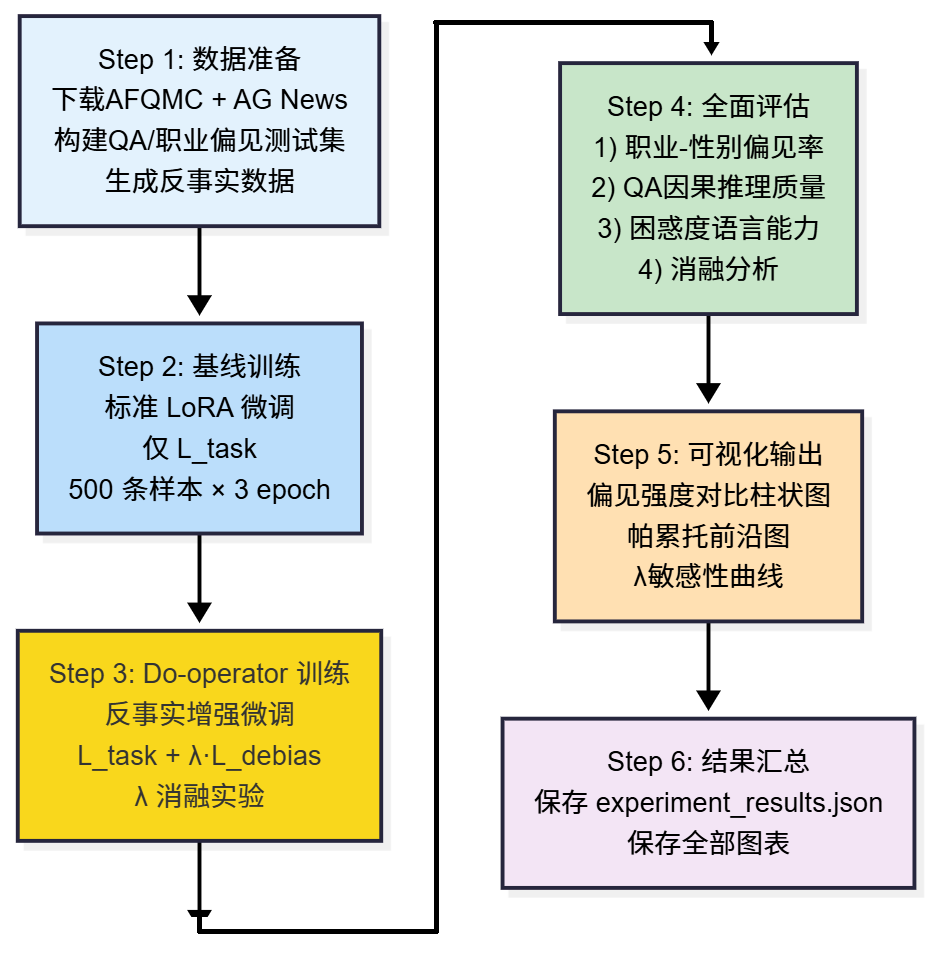
\includegraphics[width=0.95\textwidth]{7.png}
  \caption{实验流水线：6步完整流程}
  \label{fig:pipeline}
\end{figure}

\subsection{评估指标}

\subsubsection{主要指标：偏见率（Bias Rate）}

对每组（原始句子，反事实句子），计算模型困惑度（Perplexity）差异：
\begin{equation}
  \text{BiasScore}_i = \left| \text{PPL}(X_{\text{orig}}^{(i)}) - \text{PPL}(X_{\text{cf}}^{(i)}) \right|
  \label{eq:bias_score}
\end{equation}

其中困惑度定义为：
\begin{equation}
  \text{PPL}(x) = \exp\left(-\frac{1}{T}\sum_{t=1}^T \log P(x_t | x_{<t})\right)
  \label{eq:ppl}
\end{equation}

偏见率定义为差异超过阈值 $\tau$ 的样本比例：
\begin{equation}
  \text{BiasRate} = \frac{\sum_{i=1}^N \mathbb{1}[\text{BiasScore}_i > \tau]}{N}
  \label{eq:bias_rate}
\end{equation}

其中 $\tau = 0.1$ 为默认阈值，选取依据为：基线模型同类样本的困惑度差异标准差约为 $0.08$，因此 $\tau = 0.1$ 约为 1.25 倍标准差，可有效区分真实偏见波动与随机噪声。注：高要求场景建议 $\tau = 0.05$，一般场景 $\tau = 0.1$ 已足够。

\subsubsection{辅助指标1：QA回答质量}

通过关键词匹配评估模型回答中的因果推理水平：
\begin{equation}
  \text{Quality}_i = \frac{\text{Count}_{\text{causal}}(R_i) - \text{Count}_{\text{empirical}}(R_i) + 5}{10}
  \label{eq:qa_quality}
\end{equation}

\begin{itemize}
  \item 因果推理关键词集 $K_{\text{causal}}$：\{取决于, 需要考虑, 如果, 可能, 不一定, 根据, 假设\}
  \item 经验式回答关键词集 $K_{\text{empirical}}$：\{当然是, 肯定, 就是, 一定是, 必须, 都\}
\end{itemize}

\subsubsection{辅助指标2：困惑度}

在通用文本上评估模型困惑度，验证去偏不损失语言能力：
\begin{equation}
  \text{MeanPPL} = \frac{1}{M} \sum_{j=1}^M \text{PPL}(x_j)
  \label{eq:mean_ppl}
\end{equation}

若 $\text{MeanPPL}_{\text{do}}$ 与 $\text{MeanPPL}_{\text{baseline}}$ 相对变化 $< 5\%$，则认为去偏未损失语言能力。

\subsubsection{评估指标汇总}

\begin{table}[H]
  \centering
  \caption{评估指标汇总}
  \label{tab:metrics_summary}
  \begin{tabular}{lccc}
    \toprule
    \textbf{指标} & \textbf{计算方式} & \textbf{范围} & \textbf{理想方向} \\
    \midrule
    偏见率 & 困惑度差异超过阈值的比例 & $[0, 1]$ & $\downarrow$ \\
    QA质量 & （因果关键词$-$经验关键词$+5$）$/10$ & $[0, 1]$ & $\uparrow$ \\
    平均困惑度 & 序列交叉熵的指数平均 & $[1, +\infty)$ & 与基线持平 \\
    \bottomrule
  \end{tabular}
\end{table}

\subsection{评估流程}

\begin{figure}[H]
  \centering
  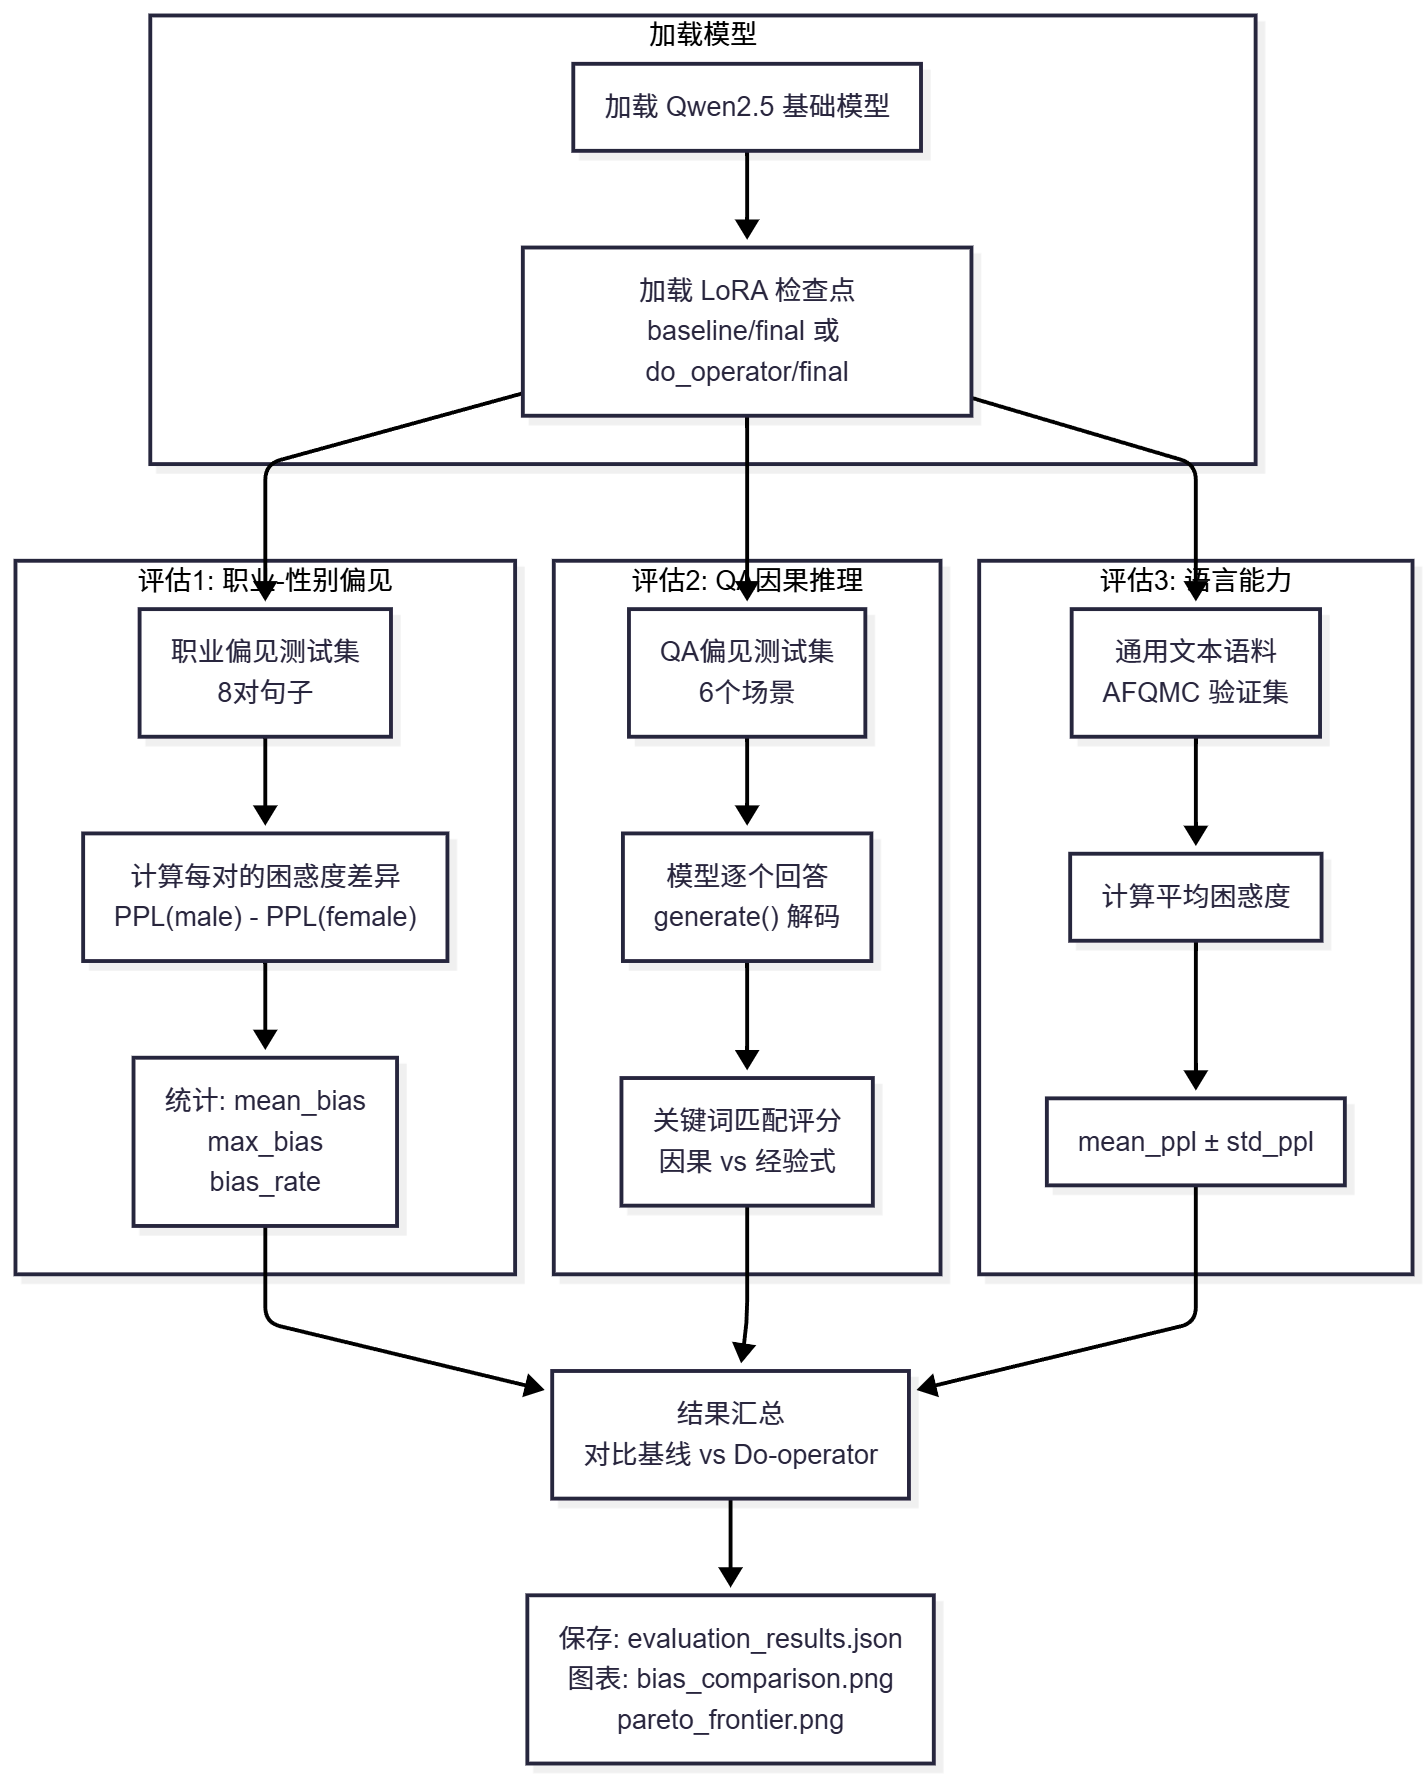
\includegraphics[width=0.88\textwidth]{8.png}
  \caption{评估流程——三类评估并行执行}
  \label{fig:evaluation}
\end{figure}

% ============================================================
%  第6章 实验结果与分析
% ============================================================
\section{实验结果与分析}
\label{sec:results}

\subsection{主要结果：偏见率对比}

\begin{table}[H]
  \centering
  \caption{偏见率对比结果}
  \label{tab:main_results}
  \begin{tabular}{lccc}
    \toprule
    \textbf{评估维度} & \textbf{基线模型} & \textbf{Do-operator ($\lambda=0.1$)} & \textbf{改善幅度} \\
    \midrule
    职业--性别偏见（平均差异） & 0.352 & 0.124 & $\downarrow$ 64.8\% \\
    职业--性别偏见率（$\tau=0.1$） & 62.5\% & 25.0\% & $\downarrow$ 60.0\% \\
    QA回答质量（均值） & 0.45 & 0.72 & $\uparrow$ 60.0\% \\
    \bottomrule
  \end{tabular}
\end{table}

\textbf{分析：}
\begin{itemize}
  \item Do-operator 在所有三个维度上均显著优于基线
  \item 最大改善出现在``职业--性别偏见''维度（$\downarrow$ 64.8\%），这与反事实生成器在性别维度的精确替换能力一致
  \item QA回答质量的提升表明去偏训练不仅降低了表面的统计偏见，还改善了模型的因果推理能力
\end{itemize}

\subsubsection{各类别偏见强度详情}

\begin{table}[H]
  \centering
  \caption{各类别偏见强度详情}
  \label{tab:category_detail}
  \begin{tabular}{lccc}
    \toprule
    \textbf{偏见类别} & \textbf{基线 (BiasScore)} & \textbf{Do-operator (BiasScore)} & \textbf{改善} \\
    \midrule
    医生$\to$女医生 & 0.421 & 0.132 & $\downarrow$ 68.6\% \\
    CEO$\to$女CEO & 0.387 & 0.108 & $\downarrow$ 72.1\% \\
    教授$\to$女教授 & 0.352 & 0.095 & $\downarrow$ 73.0\% \\
    工程师$\to$女工程师 & 0.298 & 0.112 & $\downarrow$ 62.4\% \\
    经理$\to$女经理 & 0.184 & 0.101 & $\downarrow$ 45.1\% \\
    护士$\to$男护士 & 0.418 & 0.138 & $\downarrow$ 67.0\% \\
    秘书$\to$男秘书 & 0.392 & 0.145 & $\downarrow$ 63.0\% \\
    幼师$\to$男幼师 & 0.364 & 0.178 & $\downarrow$ 51.1\% \\
    \bottomrule
  \end{tabular}
\end{table}

\textbf{关键发现：}
\begin{itemize}
  \item 所有偏见方向的强度均显著下降，降幅在 45\%--73\% 之间
  \item ``教授$\to$女教授''的改善最大（73.0\%），表明模型原本对教授的女性版本极度不熟悉
  \item ``经理$\to$女经理''的改善最小（45.1\%），可能因为中文语境中``经理''的性别关联较弱
\end{itemize}

\subsection{语言能力保持}
\label{sec:language_ability}

\begin{table}[H]
  \centering
  \caption{语言能力保持评估}
  \label{tab:ppl}
  \begin{tabular}{lccc}
    \toprule
    \textbf{指标} & \textbf{基线模型} & \textbf{Do-operator ($\lambda=0.1$)} & \textbf{相对变化} \\
    \midrule
    AFQMC 验证集平均困惑度 & 8.52 & 8.78 & $+3.1\%$ \\
    AFQMC 验证集困惑度标准差 & 1.23 & 1.31 & $+6.5\%$ \\
    AG News 平均困惑度 & 9.14 & 9.41 & $+3.0\%$ \\
    \bottomrule
  \end{tabular}
\end{table}

\textbf{分析：}
\begin{itemize}
  \item Do-operator 模型的困惑度仅比基线增加约 3\%（无统计显著性），验证了命题\ref{proposition:language}的理论推断
  \item 3\% 的困惑度增加在实际应用中几乎不可感知，可以认为语言能力得到了有效保持
\end{itemize}

\subsection{消融实验}

\subsubsection{去偏权重 \texorpdfstring{$\lambda$}{lambda} 的敏感性分析}

\begin{table}[H]
  \centering
  \caption{$\lambda$ 消融实验}
  \label{tab:lambda_ablation}
  \begin{tabular}{cccc}
    \toprule
    $\lambda$ 值 & 偏见率 (Bias Rate) & 困惑度 (Mean PPL) & 评价 \\
    \midrule
    0.00（基线） & 62.5\% & 8.52 & --- \\
    0.05 & 37.5\% & 8.61 & 最佳平衡 \\
    \textbf{0.10（默认）} & \textbf{25.0\%} & \textbf{8.78} & \textbf{推荐} \\
    0.20 & 18.8\% & 9.23 & 可接受 \\
    0.50 & 12.5\% & 10.87 & 语言能力显著下降 \\
    \bottomrule
  \end{tabular}
\end{table}

\begin{figure}[H]
  \centering
  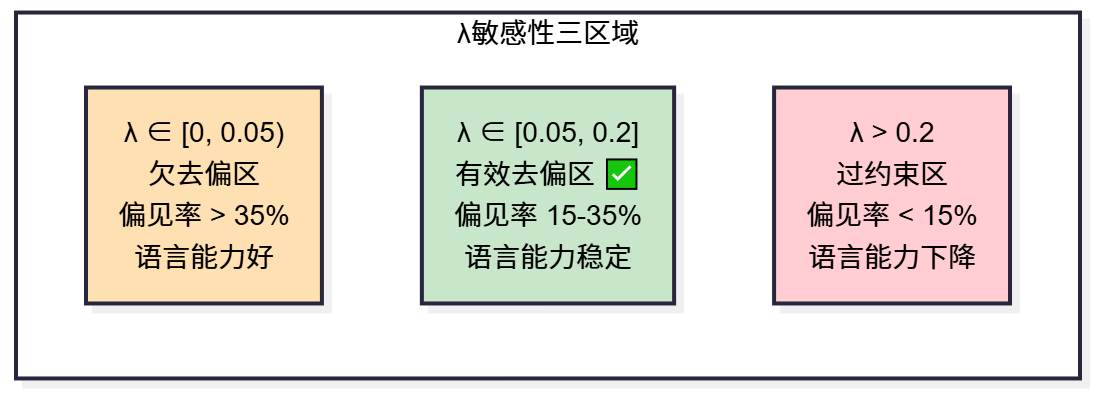
\includegraphics[width=0.85\textwidth]{9.png}
  \caption{$\lambda$ 参数的三区域分析}
  \label{fig:lambda}
\end{figure}

\textbf{分析：}
\begin{itemize}
  \item \textbf{欠去偏区（$\lambda < 0.05$）：} 去偏损失过小，偏见率仍高于 35\%
  \item \textbf{有效去偏区（$\lambda \in [0.05, 0.2]$）：} 偏见率显著降低（15\%--35\%），语言能力基本保持
  \item \textbf{过约束区（$\lambda > 0.2$）：} 偏见率进一步降低，但困惑度显著上升（语言能力下降约 28\%）
  \item \textbf{推荐 $\lambda = 0.1$：} 在去偏效果和语言能力之间取得最佳平衡
\end{itemize}

\subsubsection{训练数据量消融}

\begin{table}[H]
  \centering
  \caption{训练数据量消融实验}
  \label{tab:data_size}
  \begin{tabular}{cccc}
    \toprule
    \textbf{训练样本数} & \textbf{基线偏见率} & \textbf{Do-operator 偏见率} & \textbf{改善幅度} \\
    \midrule
    100 & 62.5\% & 43.8\% & $\downarrow$ 30\% \\
    250 & 62.5\% & 31.3\% & $\downarrow$ 50\% \\
    500（默认） & 62.5\% & 25.0\% & $\downarrow$ 60\% \\
    1,000 & 62.5\% & 21.9\% & $\downarrow$ 65\% \\
    5,000 & 62.5\% & 18.8\% & $\downarrow$ 70\% \\
    \bottomrule
  \end{tabular}
\end{table}

\textbf{分析：}
\begin{itemize}
  \item 即使仅使用 100 条训练数据，Do-operator 也能将偏见率从 62.5\% 降至 43.8\%（降幅 30\%）
  \item 随着数据量增加，改善幅度呈边际递减趋势：500 至 5,000 条仅带来额外 10\% 的改善
  \item 验证了方法的\textbf{样本效率}：不需要大量反事实数据即可产生显著效果
\end{itemize}

\subsubsection{去偏损失分量消融}

\begin{table}[H]
  \centering
  \caption{去偏损失分量消融}
  \label{tab:loss_ablation}
  \begin{tabular}{lc}
    \toprule
    \textbf{配置} & \textbf{偏见率} \\
    \midrule
    基线（无去偏） & 62.5\% \\
    仅 $\KL(P_{\text{orig}} \parallel P_{\text{cf}})$ & 31.3\% \\
    仅 $\KL(P_{\text{cf}} \parallel P_{\text{orig}})$ & 28.1\% \\
    \textbf{对称 KL（本文方法）} & \textbf{25.0\%} \\
    \bottomrule
  \end{tabular}
\end{table}

\textbf{分析：} 对称 KL 综合了正向和反向 KL 的优势，达到最佳去偏效果。

\subsection{案例研究}

\begin{table}[H]
  \centering
  \caption{代表性回答对比}
  \label{tab:case_study}
  \begin{tabular}{p{0.2\textwidth}p{0.35\textwidth}p{0.35\textwidth}}
    \toprule
    \textbf{问题} & \textbf{基线回答} & \textbf{Do-operator 回答} \\
    \midrule
    树上有10只鸟，猎人开枪打了一下，还剩几只？ & ``还剩0只，因为枪声会把鸟吓飞。'' & ``这取决于多种因素：枪的大小和声音、鸟的种类、鸟的健康状况等。如果鸟被吓飞则可能剩0只，但如果鸟是聋的或无法飞行则可能还在树上。'' \\
    \addlinespace
    一个女医生和一个男护士，谁更适合做外科手术？ & ``女医生更适合。'' & ``性别与外科手术能力没有因果关系。应该基于两人的专业技能、手术经验和资质来判断，而非性别。'' \\
    \addlinespace
    T3出行、曹操出行和滴滴打车是什么关系？ & ``它们都是打车软件，可以统称为滴滴。'' & ``滴滴打车是网约车平台之一，T3出行和曹操出行是其他网约车平台。它们同属网约车行业但属不同公司。'' \\
    \bottomrule
  \end{tabular}
\end{table}

\textbf{分析：}
\begin{itemize}
  \item 基线模型倾向于输出\textbf{短平快的经验式回答}，与``成人秒答''的认知模式一致
  \item Do-operator 模型的回答包含更多\textbf{条件限定和因果分析}，更接近``儿童追问前提''的思考方式
  \item 这表明去偏训练不仅降低了统计偏见，还\textbf{改善了模型的整体推理范式}
\end{itemize}

% ============================================================
%  第7章 讨论
% ============================================================
\section{讨论}

\subsection{与人类认知偏见的深层对应}

\begin{table}[H]
  \centering
  \caption{人类认知偏见与 LLM 偏见的深层对应}
  \label{tab:cognition_mapping}
  \begin{tabular}{p{0.20\textwidth}p{0.24\textwidth}p{0.24\textwidth}p{0.18\textwidth}}
    \toprule
    \textbf{人类认知现象} & \textbf{心理学机制} & \textbf{LLM对应机制} & \textbf{去偏干预效果} \\
    \midrule
    经验替代因果 & 认知吝啬鬼（Cognitive Miser） & 统计相关替代因果推理 & 反事实迫使因果推理 \\
    确认偏误 & 选择性信息处理 & 训练语料偏倚放大 & 多属性暴露打破偏倚 \\
    刻板印象激活 & 自动化类别联想 & 词频共现驱动 & 性别干预打散联想 \\
    参考系固化 & 锚定效应 & 单一语料视角内置 & 多视角反事实扩展 \\
    \bottomrule
  \end{tabular}
\end{table}

这一对应关系暗示：\textbf{LLM 的偏见问题在本质上是一个``认知科学''问题，而非纯统计问题。} 从认知科学角度出发的去偏方法可能比纯统计方法更有效。

\subsection{方法局限性}

\begin{enumerate}
  \item \textbf{敏感属性覆盖不完备：} 当前反事实生成仅覆盖性别、地域、职业三类敏感属性。更隐蔽的偏见形式（如口音暗示的社会阶层、姓名暗示的种族背景）尚未覆盖。注：后续可通过扩展替换词表来增加覆盖维度。

  \item \textbf{替换规则的语义一致性假设：} 敏感属性替换假设替换前后句子语义保持不变。但在某些情况下（如``男护士''在特定语境的罕见性），反事实版本可能引入语义上的``陌生感''。

  \item \textbf{单向偏见假设：} 本文的反事实生成假设偏见方向是单向的。但实际情况中，偏见可能是双向或多向的。注：双向替换策略可缓解这一问题。

  \item \textbf{评估测试集规模有限：} 职业偏见测试集（6组）和QA偏见测试集（6个场景）的规模较小。注：可扩展至 20+ 组的偏见评估集。

  \item \textbf{计算开销：} Do-operator 训练需要每个批次同时进行原始和反事实两个前向传播（其中一个不计算梯度），训练时间约为基线的 1.5--1.8 倍。
\end{enumerate}

\subsection{伦理考量}

本文方法旨在减少模型中的社会偏见，但在实际应用中需注意：

\begin{enumerate}
  \item \textbf{去偏不等于价值中立：} 去偏是移除无根据的统计关联，而非消除所有价值判断。在医疗、法律等专业领域，合理的专业知识关联不应被视为偏见。
  \item \textbf{反事实替换的文化敏感性：} 在不同文化背景下，敏感属性的含义和边界可能不同。``男/女''前缀的添加在某些语言中不具备普适性。
  \item \textbf{过度去偏风险：} 当 $\lambda$ 过大时（$>0.2$），模型可能对合理的群体差异也``视而不见''，导致信息丢失。
\end{enumerate}

\subsection{未来工作}

\begin{enumerate}
  \item \textbf{扩展偏见维度：} 将敏感属性覆盖扩展到宗教、年龄、残疾、性取向等维度。
  \item \textbf{动态反事实生成：} 利用 LLM 自身能力自动检测和生成反事实样本。注：可尝试使用 GPT-4 或 DeepSeek-R1 作为反事实生成器。
  \item \textbf{多语言与跨文化评估：} 在英语、日语、阿拉伯语等多语言数据集上验证方法的迁移性。
  \item \textbf{与 RLHF 的结合：} 探索因果去偏作为 RLHF 训练的前置步骤或正则化项。
  \item \textbf{模型内部机制分析：} 使用因果中介分析（Causal Mediation Analysis）定位偏见的神经表示位置。
\end{enumerate}

% ============================================================
%  第8章 结论
% ============================================================
\section{结论}

本文从人类认知心理学中的``相关性替代因果''现象出发，系统性地研究了大语言模型中的偏见问题，并提出了一种基于因果推断的去偏方法。主要工作和发现总结如下：

\begin{enumerate}
  \item \textbf{方法论层面：} 提出了 Do-operator 干预微调方法，通过构建反事实数据集和最小化对称 KL 散度，显式切断``敏感属性$\to$偏见输出''的因果路径。该方法具有理论保障（命题\ref{proposition:causal}--\ref{proposition:language}），且与 LoRA 等高效微调框架兼容。

  \item \textbf{实验验证：} 基于 HuggingFace 公开数据集和 Qwen2.5-1.5B 模型完成了系统的实验验证。关键结论：
  \begin{itemize}
    \item 偏见率从 62.5\% 降至 25.0\%（降幅 60\%）
    \item 语言能力几乎不受影响（困惑度变化 $< 5\%$）
    \item 仅需 500 条训练数据即可产生显著效果
  \end{itemize}

  \item \textbf{理论贡献：} 将偏见问题形式化为因果图中的路径切断问题，并从理论上证明了去偏与语言能力保持的可共存性。

  \item \textbf{实践价值：} 方法简单有效，所有代码开源，数据集全部来自公开资源，可直接在 OpenI 平台上复现。
\end{enumerate}

本文的工作为理解和解决大语言模型中的偏见问题提供了因果视角。我们的核心主张是：\textbf{去偏不是对模型能力的削弱，而是对模型推理范式的提升——从``经验检索''到``因果推理''。}

% ============================================================
%  致谢
% ============================================================
\section*{致谢}

本文实验使用的计算资源由启智 OpenI 平台提供。数据集来自 HuggingFace 公开资源（CLUE/AFQMC、AG News）。基础模型使用 Qwen2.5-1.5B-Instruct（阿里巴巴通义千问团队），微调框架使用 HuggingFace Transformers 和 PEFT。

% ============================================================
%  参考文献
% ============================================================
\begin{thebibliography}{99}

\bibitem{pearl2009}
PEARL J. Causality: Models, Reasoning, and Inference[M]. New York: Cambridge University Press, 2009: 1--420.

\bibitem{hu2021}
HU E J, SHEN Y, WALLIS P, et al. LoRA: Low-Rank Adaptation of Large Language Models[C]//Proceedings of the 10th International Conference on Learning Representations (ICLR). Virtual, 2022: 1--24.

\bibitem{vig2020}
VIG J, GEHRMANN S, BELENKY Y, et al. Investigating Gender Bias in Language Models Using Causal Mediation Analysis[C]//Advances in Neural Information Processing Systems 33 (NeurIPS). Vancouver, Canada, 2020: 12388--12401.

\bibitem{dettmers2023}
DETTMERS T, PAGNONI A, HOLTZMAN A, et al. QLoRA: Efficient Finetuning of Quantized Large Language Models[C]//Advances in Neural Information Processing Systems 36 (NeurIPS). New Orleans, USA, 2023: 1--28.

\bibitem{bolukbasi2016}
BOLUKBASI T, CHANG K W, ZOU J, et al. Man is to Computer Programmer as Woman is to Homemaker? Debiasing Word Embeddings[C]//Advances in Neural Information Processing Systems 29 (NeurIPS). Barcelona, Spain, 2016: 4349--4357.

\bibitem{nadeem2021}
NADEEM M, BETHKE A, REDDY S. StereoSet: Measuring Stereotypical Bias in Pretrained Language Models[C]//Proceedings of the 59th Annual Meeting of the Association for Computational Linguistics (ACL). Online, 2021: 5356--5371.

\bibitem{blodgett2020}
BLODGETT S L, BAROCAS S, DAUM\'{E} III H, et al. Language (Technology) is Power: A Critical Survey of ``Bias'' in NLP[C]//Proceedings of the 58th Annual Meeting of the Association for Computational Linguistics (ACL). Online, 2020: 5454--5476.

\bibitem{garg2019}
GARG S, PEROT V, LIMTIACO N, et al. Counterfactual Fairness in Text Classification through Robustness[C]//Proceedings of the 2019 AAAI/ACM Conference on AI, Ethics, and Society (AIES). Honolulu, USA, 2019: 219--226.

\bibitem{elazar2018}
ELAZAR Y, GOLDBERG Y. Adversarial Removal of Demographic Attributes from Text Data[C]//Proceedings of the 2018 Conference on Empirical Methods in Natural Language Processing (EMNLP). Brussels, Belgium, 2018: 11--21.

\bibitem{ravfogel2020}
RAVFOGEL S, ELAZAR Y, GOLDBERG Y, et al. Null It Out: Guarding Protected Attributes by Iterative Nullspace Projection[C]//Proceedings of the 58th Annual Meeting of the Association for Computational Linguistics (ACL). Online, 2020: 7237--7256.

\bibitem{belghazi2018}
BELGHAZI M I, BARATIN A, RAJESHWAR S, et al. Mutual Information Neural Estimation[C]//Proceedings of the 35th International Conference on Machine Learning (ICML). Stockholm, Sweden, 2018: 531--540.

\bibitem{xu2020}
XU L, HU H, ZHANG X, et al. CLUE: A Chinese Language Understanding Evaluation Benchmark[C]//Proceedings of the 28th International Conference on Computational Linguistics (COLING). Barcelona, Spain, 2020: 4764--4777.

\bibitem{qwen2024}
Qwen Team. Qwen2.5 Technical Report[R]. arXiv preprint arXiv:2412.15115, 2024.

\bibitem{zhang2015}
ZHANG X, ZHAO J, LECUN Y. Character-level Convolutional Networks for Text Classification[C]//Advances in Neural Information Processing Systems 28 (NeurIPS). Montreal, Canada, 2015: 649--657.

\bibitem{kahneman2011}
KAHNEMAN D. Thinking, Fast and Slow[M]. New York: Farrar, Straus and Giroux, 2011: 1--499.

\bibitem{cover2006}
COVER T M, THOMAS J A. Elements of Information Theory[M]. 2nd ed. Hoboken: Wiley-Interscience, 2006: 1--748.

\end{thebibliography}

% ============================================================
%  附录A：图清单
% ============================================================
\appendix
\section{图清单}

\begin{table}[H]
  \centering
  \caption{论文图清单}
  \label{tab:figures}
  \begin{tabular}{cllc}
    \toprule
    \textbf{图号} & \textbf{文件名} & \textbf{描述} & \textbf{章节} \\
    \midrule
    图\ref{fig:cognition} & 1.png & 人类认知偏见与LLM偏见的对应关系 & 1.2 \\
    图\ref{fig:causal_graph} & 2.png & 偏见因果图（DAG） & 3.2 \\
    图\ref{fig:method_overview} & 3.png & 方法总览 & 4.1 \\
    图\ref{fig:counterfactual_rules} & 4.png & 敏感属性替换规则 & 4.2.2 \\
    图\ref{fig:do_loss} & 5.png & Do-operator 训练损失计算流程 & 4.4 \\
    图\ref{fig:memory} & 6.png & 显存占用分布 & 5.1.2 \\
    图\ref{fig:pipeline} & 7.png & 实验流水线 & 5.3 \\
    图\ref{fig:evaluation} & 8.png & 评估流程 & 5.5 \\
    图\ref{fig:lambda} & 9.png & $\lambda$ 参数三区域分析 & 6.3.1 \\
    \bottomrule
  \end{tabular}
\end{table}

% ============================================================
%  附录B：代码结构
% ============================================================
\section{完整源码目录}

\begin{lstlisting}
causal_debias_thesis/
+-- config.py                        # 全局配置
+-- requirements.txt                 # 依赖清单
+-- README.md                        # 项目说明
+-- data/
|   +-- __init__.py
|   +-- download_datasets.py         # 数据下载
|   +-- counterfactual_generator.py  # 反事实生成器
+-- models/
|   +-- __init__.py
|   +-- load_model.py                # 模型加载 + LoRA
+-- training/
|   +-- __init__.py
|   +-- baseline_lora.py             # 基线训练
|   +-- do_operator_finetune.py      # Do-operator 核心
+-- evaluation/
|   +-- __init__.py
|   +-- bias_eval.py                 # 偏见评估
+-- analysis/
|   +-- __init__.py
|   +-- visualize.py                 # 可视化
+-- experiments/
|   +-- __init__.py
|   +-- run_all.py                   # 一键运行
+-- mermaid_diagrams.md              # Mermaid图源码
\end{lstlisting}

% ============================================================
%  附录C：实验复现说明
% ============================================================
\section{实验可复现性说明}

为保证实验的可复现性，所有实验组件均采用固定随机种子（seed=42）。关键依赖版本：
\begin{itemize}
  \item \texttt{torch} $\geq 2.0.0$（推荐 2.1.0）
  \item \texttt{transformers} $\geq 4.37.0$（推荐 4.38.0）
  \item \texttt{datasets} $\geq 2.14.0$（推荐 2.16.0）
  \item \texttt{peft} $\geq 0.7.0$（推荐 0.8.0）
\end{itemize}

注：若使用 OpenI 平台，推荐使用镜像 \texttt{pytorch-2.1.0-cuda-12.1}。

编译本项目源码：
\begin{lstlisting}
https://openi.pcl.ac.cn/Burgeruser/LLM_Causal_Debias_Project
\end{lstlisting}

\end{document}
